%%%% SEITENRAENDER, SCHRIFTGROESSE UND ZEILENABSTAND NICHT ABAENDERN => SONST GIBT ES PUNKTEABZUG
\documentclass[a4paper,11pt,singlespacing]{article}
% \usepackage[left=2.5cm,right=2.5cm,top=2.5cm]{geometry}
\usepackage{setspace}
\usepackage[utf8]{inputenc}
\usepackage{graphicx}
\usepackage{color}
\usepackage{hyperref}
\usepackage{biblatex}
\usepackage{listings}
\usepackage{xcolor}

\definecolor{codegreen}{rgb}{0,0.6,0}
\definecolor{codegray}{rgb}{0.5,0.5,0.5}
\definecolor{codepurple}{rgb}{0.58,0,0.82}
\definecolor{backcolour}{rgb}{0.95,0.95,0.92}

\lstdefinestyle{mystyle}{
    backgroundcolor=\color{backcolour},   
    commentstyle=\color{codegreen},
    keywordstyle=\color{magenta},
    numberstyle=\tiny\color{codegray},
    stringstyle=\color{codepurple},
    basicstyle=\ttfamily\footnotesize,
    breakatwhitespace=false,         
    breaklines=true,                 
    captionpos=b,                    
    keepspaces=true,                 
    numbers=left,                    
    numbersep=5pt,                  
    showspaces=false,                
    showstringspaces=false,
    showtabs=false,                  
    tabsize=2
}

\lstset{style=mystyle}

\addbibresource{sample.bib}


\usepackage{listings,xcolor}
%opening
\title{Project title}
\author{
	Name Mat.No.
	}


\begin{document}
% Absatzeinrückung verhindern
\setlength{\parindent}{0ex}


\begin{titlepage}
	
	\newcommand{\HRule}{\rule{\linewidth}{0.5mm}} % Defines a new command for the horizontal lines, change thickness here
	
	\center % Center everything on the page
	
	%----------------------------------------------------------------------------------------
	%	HEADING SECTIONS
	%----------------------------------------------------------------------------------------
	
	\textsc{\LARGE University of Applied Sciences Ravensburg Weingarten}\\[1.5cm] % Name of your university/college
	\textsc{\Large Department of
		Electrical Engineering
		and Computer Science}\\[0.5cm] % Major heading such as course name
	\textsc{\large Computer Science Project}\\[0.5cm] % Minor heading such as course title
	
	%----------------------------------------------------------------------------------------
	%	TITLE SECTION
	%----------------------------------------------------------------------------------------
	
	\HRule \\[0.4cm]
	{ \huge \bfseries Prototype of a autonomous selfi drone utilizing pose estimation}\\[0.4cm] % Title of your document
	\HRule \\[1.5cm]
	
	%----------------------------------------------------------------------------------------
	%	AUTHOR SECTION
	%----------------------------------------------------------------------------------------
	
	\begin{minipage}{0.4\textwidth}
		\begin{flushleft} \large
			\emph{Author:}\\
			Felix \textsc{Hamburger}\\ % Your name
			28403
		\end{flushleft}
	\end{minipage}
	~
	\begin{minipage}{0.4\textwidth}
		\begin{flushright} \large
			\emph{Supervisor:} \\
			Prof. Dr. Markus \textsc{Schneider} % Supervisor's Name
		\end{flushright}
	\end{minipage}\\[2cm]

	% If you don't want a supervisor, uncomment the two lines below and remove the section above
	%\Large \emph{Author:}\\
	%John \textsc{Smith}\\[3cm] % Your name
	
	%----------------------------------------------------------------------------------------
	%	DATE SECTION
	%----------------------------------------------------------------------------------------
	
	{\large \today}\\[5cm] % Date, change the \today to a set date if you want to be precise
	
	%----------------------------------------------------------------------------------------
	%	LOGO SECTION
	%----------------------------------------------------------------------------------------
	
	
	
\includegraphics[width=7cm]{images/logo.png} % Include a department/university logo - this will require the graphicx package
	
	%----------------------------------------------------------------------------------------
	
	\vfill % Fill the rest of the page with whitespace
	
\end{titlepage}


\tableofcontents
\pagebreak



\section{Introduction}
The world is growing fast

\cite{tello_idea}

\section{Requirements}
\subsection{Mediapipe}
\subsection{djitellopy}
\subsection{Drone}

The drone used for this project is the tello drone from dji with the following technical details:

\begin{figure}[h!]
	\centering
	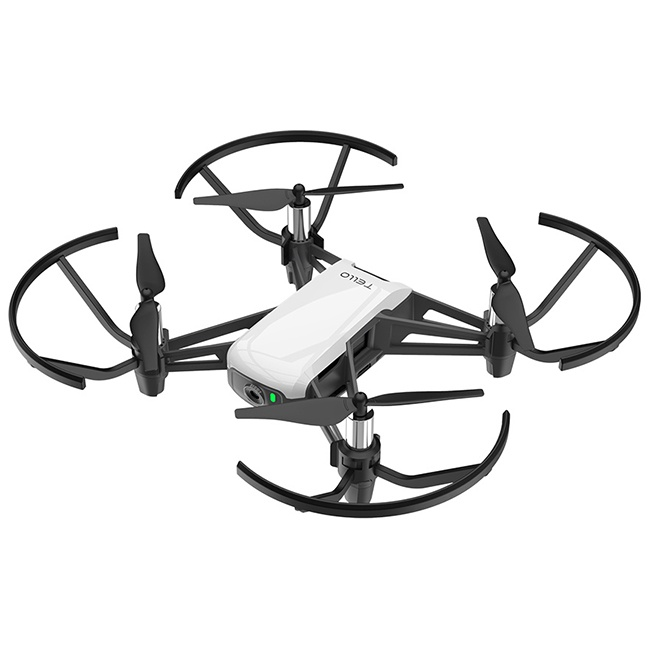
\includegraphics[scale=0.5]{images/tello_front.jpeg}
	\caption{Tello Drone}
	\label{tello_drone}
\end{figure}

\begin{center}
	\begin{tabular}{ l  l} 
	\hline
	 \textbf{Aircraft:} & Weight: 80g\\
	 & Dimensions: 98×92.5×41 mm  \\
	 & Propeller: 7,62cm\\
	 & Built-in Functions: Range Finder,\\
	 & Barometer, LED, Vision System,\\
	 & 2.4 GHz 802.11n Wi-Fi, 720p Live View\\
	 & Port: Micro USB Charging Port\\\\
	 \hline
	\\
	 \textbf{Flight Performance:} & Max Flight Distance: 100m\\
	 & Max Speed: 8m/s\\
	 & Max Flight Time: 13min\\
	 & Max Flight Height: 30m\\\\
	 \hline
	 \\
	 \textbf{Battery:} & Detachable Battery: 1.1Ah/3.8V\\\\
	 \hline
	 \\
	 \textbf{Camera:} & Photo: 5MP (2592x1936)\\
	 & FOV: 82.6° \\
	 & Video: HD720P30\\
	 & Format: JPG(Photo); MP4(Video)\\
	 & Electric Image Stabilization: Yes\\
	 \hline
	\end{tabular}
\end{center}

\section{Implementation}

\section{Conclusion}
\section{Improvements}


\pagebreak
\listoffigures
\pagebreak
\printbibliography[heading=bibintoc]
\pagebreak
\lstlistoflistings
\pagebreak
\lstinputlisting[language=Python,caption=Main.py]{../../source/Main.py}
\lstinputlisting[language=Python,caption=Controller.py]{../../source/Controller.py}
\lstinputlisting[language=Python,caption=Constants.py]{../../source/Constants.py}
\lstinputlisting[language=Python,caption=PoseDetection.py]{../../source/PoseDetection.py}
\end{document}